%%%%%%%%%%%%%%%%%%%%%%%%%%%%%%%%%%%%%%%%%
% NIWeek 2014 Poster by T. Reveyrand
% www.microwave.fr
% http://www.microwave.fr/LaTeX.html
% ---------------------------------------
% 
% Original template created by:
% Brian Amberg (baposter@brian-amberg.de)
%
% This template has been downloaded from:
% http://www.LaTeXTemplates.com
%
% License:
% CC BY-NC-SA 3.0 (http://creativecommons.org/licenses/by-nc-sa/3.0/)
%
%%%%%%%%%%%%%%%%%%%%%%%%%%%%%%%%%%%%%%%%%

%----------------------------------------------------------------------------------------
%   PACKAGES AND OTHER DOCUMENT CONFIGURATIONS
%----------------------------------------------------------------------------------------

\documentclass[a0paper,portrait]{baposter}

\usepackage[font=small,labelfont=bf]{caption} % Required for specifying captions to tables and figures
\usepackage{booktabs} % Horizontal rules in tables
\usepackage{relsize} % Used for making text smaller in some places

\usepackage{amsmath,amsfonts,amssymb,amsthm} % Math packages
\usepackage{eqparbox}

\usepackage{textcomp}

\usepackage{caption}
\usepackage{subcaption}
\usepackage{graphicx}
%\usepackage{hyperref}

\graphicspath{{figures/}} % Directory in which figures are stored

 \definecolor{bordercol}{RGB}{40,40,40} % Border color of content boxes
 \definecolor{headercol1}{RGB}{186,215,230} % Background color for the header in the content boxes (left side)
 \definecolor{headercol2}{RGB}{120,120,120} % Background color for the header in the content boxes (right side)
 \definecolor{headerfontcol}{RGB}{0,0,0} % Text color for the header text in the content boxes
 \definecolor{boxcolor}{RGB}{210,235,250} % Background color for the content in the content boxes


\begin{document}

\background{ % Set the background to an image (background.pdf)
\begin{tikzpicture}[remember picture,overlay]
\draw (current page.north west)+(-2em,2em) node[anchor=north west]
{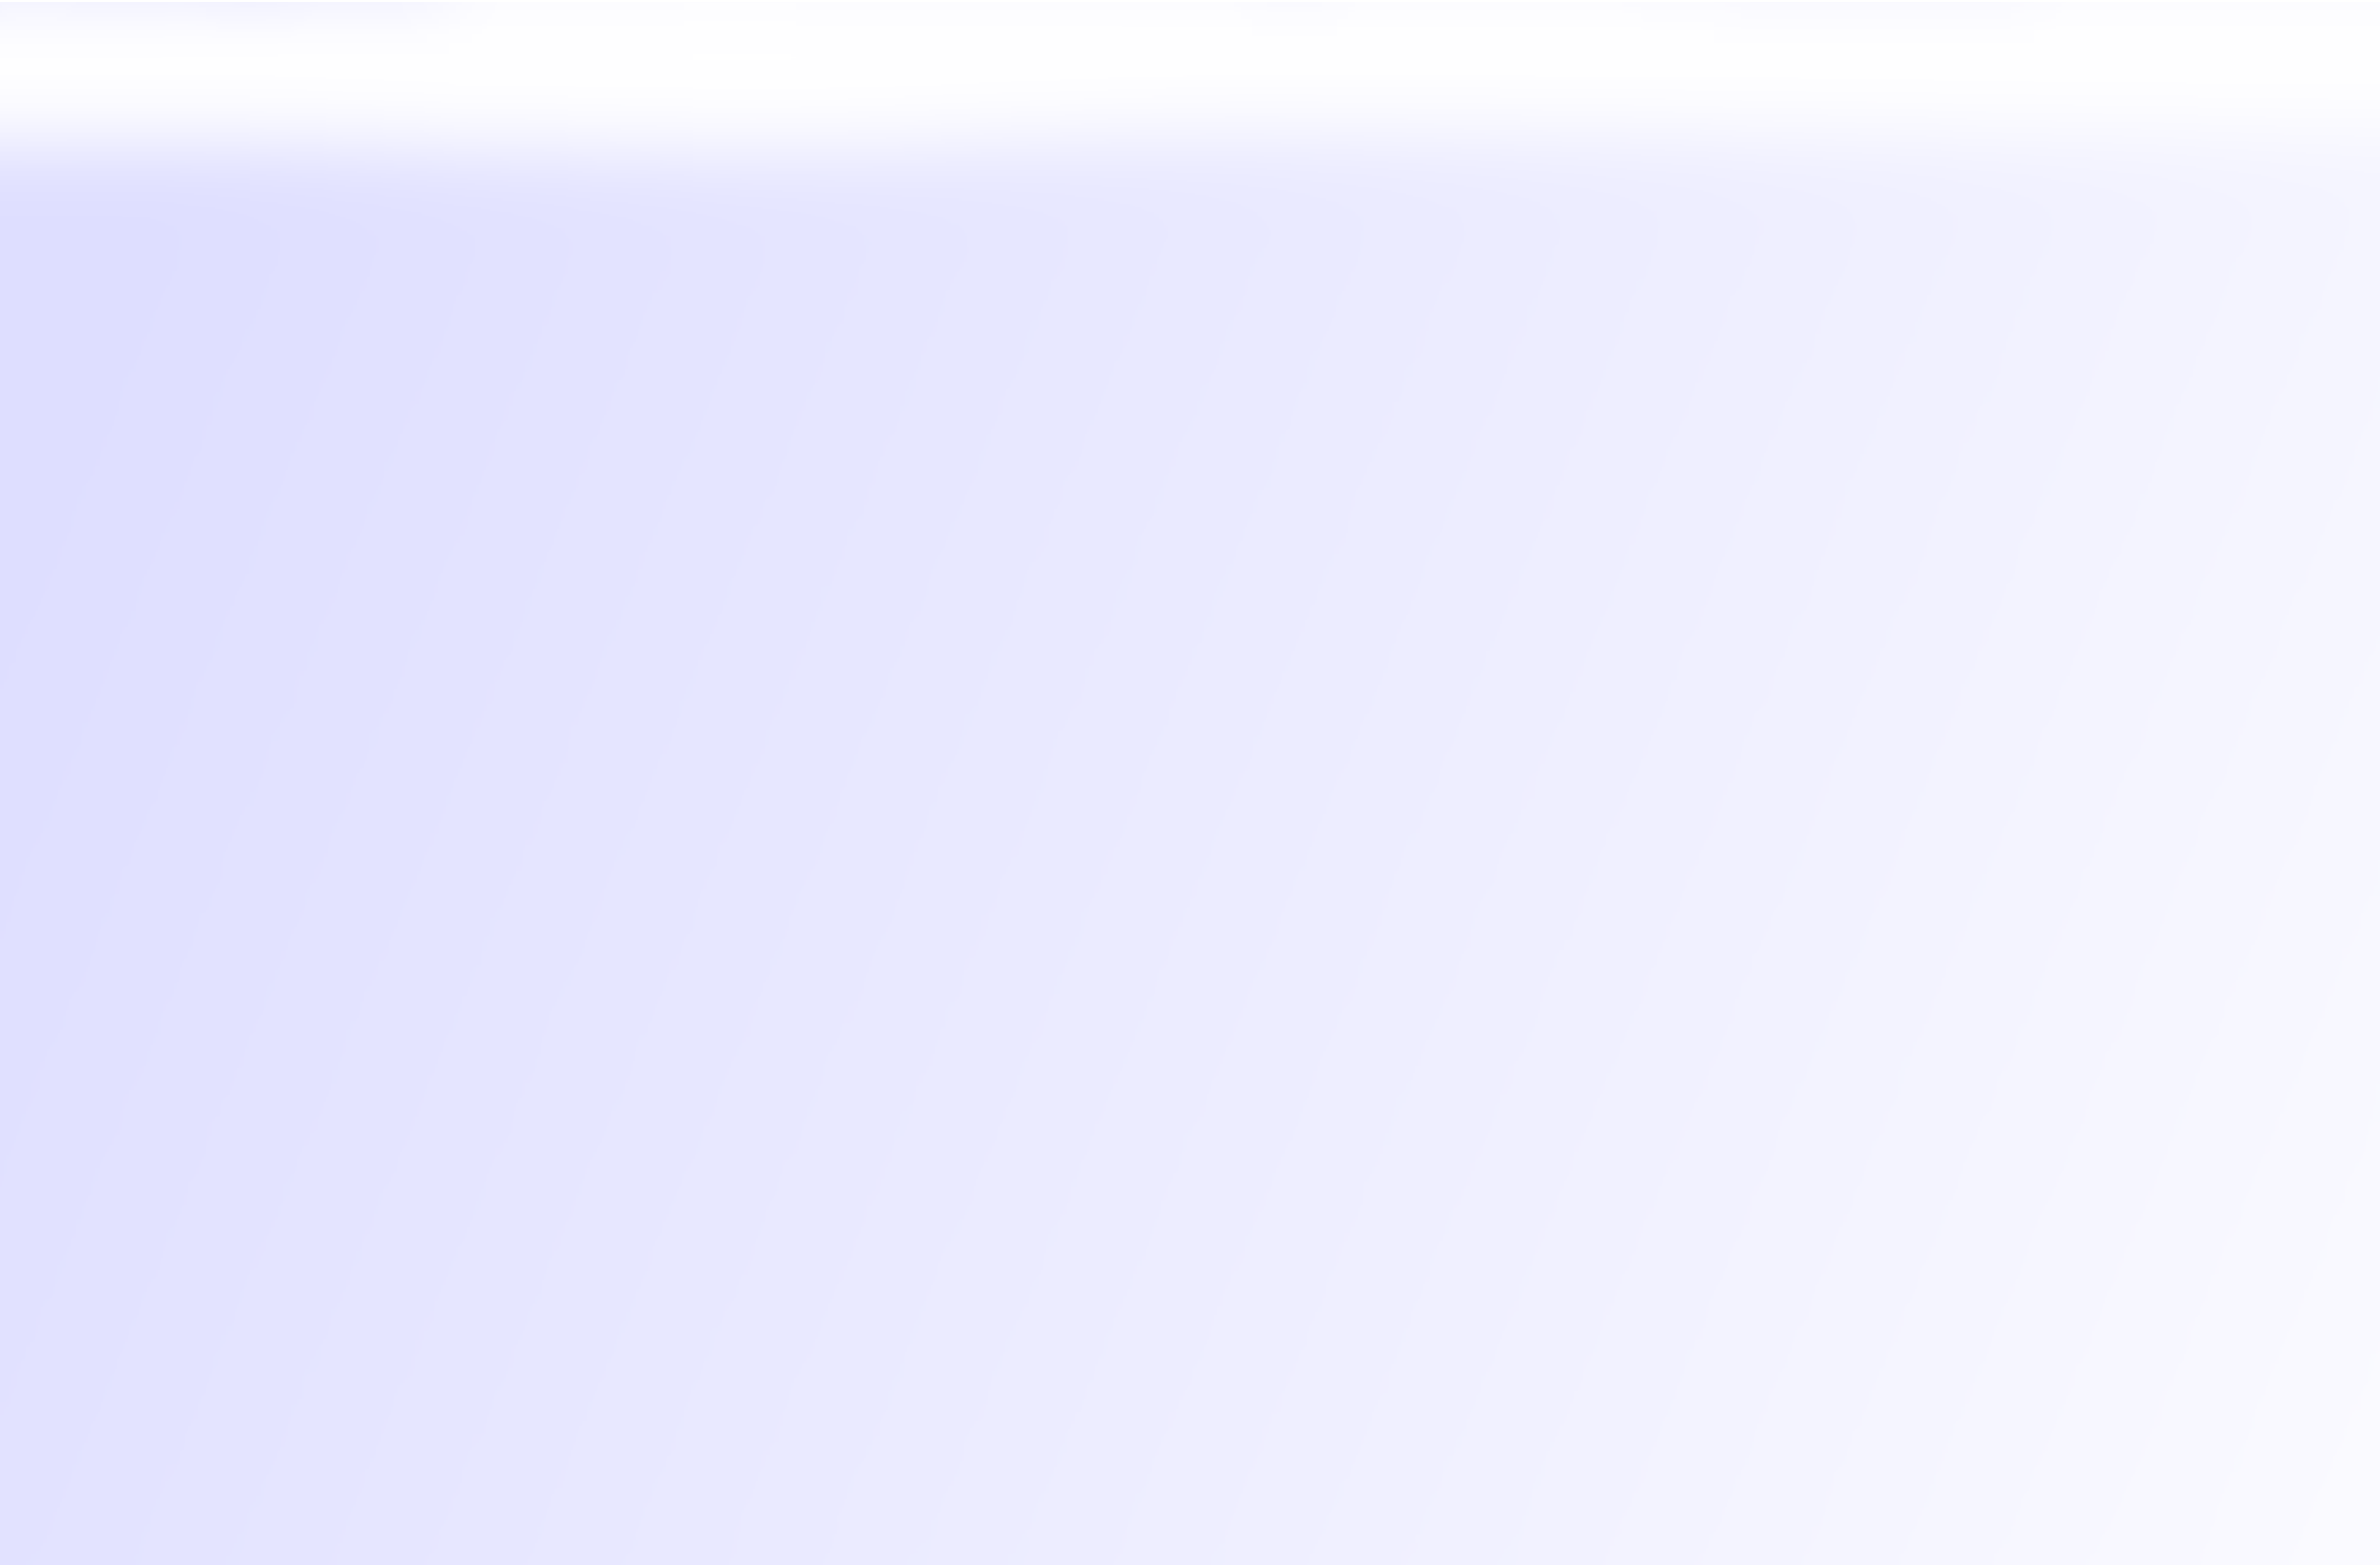
\includegraphics[height=1.1\textheight]{background}};
\end{tikzpicture}
}

\begin{poster}{
grid=false,
columns=4,
borderColor=bordercol, % Border color of content boxes
headerColorOne=headercol1, % Background color for the header in the content boxes (left side)
headerColorTwo=headercol2, % Background color for the header in the content boxes (right side)
headerFontColor=headerfontcol, % Text color for the header text in the content boxes
boxColorOne=boxcolor, % Background color for the content in the content boxes
headershape=roundedright, % Specify the rounded corner in the content box headers
headerfont=\Large\sf\bf, % Font modifiers for the text in the content box headers
textborder=rectangle,
background=none,
headerborder=open, % Change to closed for a line under the content box headers
boxshade=plain
}
{
\includegraphics[width=3cm]{BiAtA2017.png}} %to do change to grades-nda 2018
%
%----------------------------------------------------------------------------------------
%   TITLE AND AUTHOR NAME
%----------------------------------------------------------------------------------------
%
{ \bf  \huge {Context-Free Path Querying by Matrix Multiplication} \\  \Large \it Matrix-based algorithm for graph structured data analysis} % Poster title
{\vspace{0.3em} \smaller Rustam Azimov$^1$, Semyon Grigorev$^1$,  \\  % Author names
\smaller \it $^1${Saint Petersburg State University, JetBrains, St. Petersburg, Russia } \\ % Author email addresses
\smaller  {\textbf{E-mails:} st013567@student.spbu.ru, s.v.grigoriev@spbu.ru}}
{
\includegraphics[width=3cm]{SPbGU_Logo.png}} % University/lab logo


%----------------------------------------------------------------------------------------
%   INTRODUCTION
%----------------------------------------------------------------------------------------
\headerbox{Motivation}{name=introduction,column=0,row=0, span=2}{
Context-free path querying is a technique, which recently gains
popularity in many areas, for example, graph databases, bioinformatics,
static analysis, etc. In some of these areas, it is often required
to query large graphs, and existing algorithms demonstrate
a poor performance in this case. The generalization of matrix-based
Valiant's context-free language recognition algorithm for graph
case is widely considered as a recipe for efficient context-free path
querying; however, no progress has been made in this direction so
far.

We propose the first generalization of matrix-based Valiant's algorithm
for context-free path querying. Our generalization does not
deliver a truly sub-cubic worst-case complexity algorithm, whose
existence still remains a hard open problem in the area. On the
other hand, the utilization of matrix operations (such as matrix
multiplication) in the process of context-free path query evaluation
makes it possible to efficiently apply a wide class of optimizations
and computing techniques, such as GPGPU (General-Purpose computing
on Graphics Processing Units), parallel processing, sparse
matrix representation, distributed-memory computation, etc. Indeed,
the evaluation on a set of conventional benchmarks shows,
that our algorithm outperforms the existing ones.

}

\headerbox{Results}{name=results,column=2,row=0, span=2}{
\begin{itemize} 
\item We propose the matrix-based algorithm for context-free path querying.
\vspace{-0.2cm}
\item We implemented this algorithm with a number of optimizations and applied these implementations to the navigation query problem for some popular ontologies, taken from~\cite{RDF}.
\vspace{-0.2cm}
\item We also compared the performance of our implementations 
with the fastest analog from~\cite{GLL}.
\end{itemize}

\begin{center}
\textbf{Performance comparison of CF path querying algorithms}
\begin{itemize} 
\item sCPU (sparse CPU)~--- an implementation of our algorithm using the CSR format for sparse matrix representation and a CPU for matrix operation calculation. For sparse matrix representation in CSR format we used the Math.Net Numerics package.
\vspace{-0.2cm}
\item sGPU (sparse GPU)~--- an implementation of our algorithm using the CSR format for sparse matrix representation and a GPU for matrix operation calculation. For calculations of the matrix operations on a GPU, where matrices represented in a CSR format, we used a wrapper for the CUSPARSE library from the managedCuda library.
\end{itemize}
\textbf{Query 1} is based on the grammar $G$ for retrieving the concepts on the same layer. The running time of the algorithms is presented in ms.
	
	\begin{tabular}{ | c | c | c | c | c | c | c |}
		\hline
		Ontology & V & E & \#results & GLL & sCPU & sGPU\\
		\hline 
		\hline
		skos        & 144 & 323 & 810 & 10 & 14 & 12\\
		generations & 129 & 351 & 2164 & 19 & 20 & 13\\
		travel      & 131 & 397 & 2499 & 24 & 22 & 30\\
		univ-bench  & 179 & 413 & 2540 & 25 & 25 & 15\\
		atom-primitive & 291 & 685 & 15454 & 255 & 92 & 22\\
		biomedical & 341 & 711 & 15156 & 261 & 113 & 20\\
		foaf        & 256 & 815 & 4118 & 39 & 48 & 9\\
		people-pets & 337 & 834 & 9472 & 89 & 142 & 32\\
		funding     & 778 & 1480 & 17634 & 212 & 447 & 36\\
		wine        & 733 & 2450 & 66572 & 819 & 797 & 54\\
		pizza       & 671 & 2604 & 56195 & 697 & 430 & 24\\
		$g_{1}$     & 6224 & 11840 & 141072 & 1926 & 26957 & 82\\
		$g_{2}$     & 5864 & 19600 & 532576 & 6246 & 46809 & 185\\
		$g_{3}$     & 5368 & 20832 & 449560 & 7014 & 24967 & 127\\
		\hline
	\end{tabular}

\vspace{0.2cm}
\textbf{Query 2} is based on the grammar $G^2_S$ for retrieving concepts on the adjacent layers.
\begin{tabular}{ | c | c | c | c | c | c | c |}
	\hline
	Ontology & V & E & \#results & GLL & sCPU & sGPU\\
	\hline 
	\hline
	skos        & 144 & 323 & 1 & 1 & 2 & 1\\
	generations & 129 & 351 & 0 & 1 & 2 & 0\\
	travel      & 131 & 397 & 63 & 1 & 7 & 10\\
	univ-bench  & 179 & 413 & 81 & 11 & 15 & 9\\
	atom-primitive & 291 & 685 & 122 & 66 & 9 & 2\\
	biomedical & 341 & 711 & 2871 & 45 & 91 & 24\\
	foaf        & 256 & 815 & 10 & 2 & 14 & 3\\
	people-pets & 337 & 834 & 37 & 3 & 38 & 6\\
	funding     & 778 & 1480 & 1158 & 23 & 344 & 27\\
	wine        & 733 & 2450 & 133 & 8 & 179 & 6\\
	pizza       & 671 & 2604 & 1262 & 29 & 258 & 23\\
	$g_{1}$     & 6224 & 11840 & 9264 & 167 & 21115 & 38\\
	$g_{2}$     & 5864 & 19600 & 1064 & 46 & 10874 & 21\\
	$g_{3}$     & 5368 & 20832 & 10096 & 393 & 15736 & 40\\
	\hline
\end{tabular}
\end{center}
}
    
\headerbox{Future Research}{name=future,column=2,below=results, span=2}{
\begin{itemize} 
\item Currently, we are working on the matrix-based algorithm for path querying with conjunctive grammars which have more expressive power, than context-free grammars.
\vspace{-0.2cm}
\item We want to find new applications for path querying techniques and implement required tools.
\end{itemize}
}

\headerbox{Context-free path querying}{name=CFParsing,span=2,column=0,row=1,below=introduction}{

}

\headerbox{Matrix-based approach}
{name=app1,column=0,span=2, below=CFParsing}
{ % To reduce this block to 1 column width, remove 'span=2'
}


%----------------------------------------------------------------------------------------
%   REFERENCES
%----------------------------------------------------------------------------------------

\headerbox{References}{name=references,column=0,span=2,below=app1}{

\smaller % Reduce the font size in this block
\renewcommand{\section}[2]{\vskip 0.05em} % Get rid of the default "References" section title
%\nocite{*} % Insert publications even if they are not cited in the poster

\bibliographystyle{unsrt}
\bibliographystyle{IEEEtran}
\bibliography{biblio} % Use biblio.bib as the bibliography file
}


\headerbox{Acknowledgments}{name=ack,column=2,span=1,below=future}{
The research was supported by the Russian Science Foundation grant 18-11-00100 and a grant from JetBrains Research.
\vspace{0.15cm}
}

\headerbox{Information}{name=info,column=3,span=1,below=future}{
All materials available on GitHub: \small{https://github.com/YaccConstructor}
\vspace{0.57cm}
}


\end{poster}

\end{document}